\documentclass[runningheads]{llncs}

% Default fixed font does not support bold face
\DeclareFixedFont{\ttb}{T1}{txtt}{bx}{n}{10} % for bold
\DeclareFixedFont{\ttm}{T1}{txtt}{m}{n}{10}  % for normal

\usepackage{xcolor}
\usepackage{listings}
\usepackage{hyperref}
\usepackage{graphicx}
\usepackage{mdframed}
\usepackage{amsmath}
\usepackage{float}
\usepackage{pdfpages}

\definecolor{deepblue}{rgb}{0,0,0.5}
\definecolor{deepred}{rgb}{0.6,0,0}
\definecolor{deepgreen}{rgb}{0,0.5,0}

\hypersetup{
    colorlinks,
    citecolor=black,
    filecolor=black,
    linkcolor=black,
    urlcolor=black
}

% Python style for highlighting
\newcommand\pythonstyle{\lstset{
language=Python,
basicstyle=\ttm,
otherkeywords={self},             % Add keywords here
keywordstyle=\ttb\color{deepblue},
emph={MyClass,__init__},          % Custom highlighting
emphstyle=\ttb\color{deepred},    % Custom highlighting style
stringstyle=\color{deepgreen},
frame=tb,                         % Any extra options here
showstringspaces=false            % 
}}

% Python environment
\lstnewenvironment{python}[1][]
{
\pythonstyle
\lstset{#1}
}
{}

% Python for external files
\newcommand\pythonexternal[2][]{{
\pythonstyle
\lstinputlisting[#1]{#2}}}

% Python for inline
\newcommand\pythoninline[1]{{\pythonstyle\lstinline!#1!}}

\title{COMP472 - Reports}
\author{Thomas Backs\inst{1} \and Marco Tropiano\inst{2}\and Earl Aromin Steven\inst{3}}
\authorrunning{T. Backs, M. Tropiano \& E. Armoin}
\institute{27554524 - thomasbacks@gmail.com \and 26789331 - tropiano.m@gmail.com \and 40004997 - earlaromin@gmail.com} 

\begin{document}
    \maketitle
    \section{Introduction}
    This project is completed within the COMP 472 course. It aims is to create an unsupervised machine learning program that will take some people feedback on various items they purchased and to classify it in two different group: Positive review or negative review. We used 80\% of the data collected to train our machine, and the remaining 20\% to test our machine. The analysis of each task of the project are shown in different section.
    \section{Task 1 Analysis}
    For the task 1, we created a function called \pythoninline{def train_nb(documents, labels)}, it takes two parament which are the \pythoninline{documents} and the \pythoninline{labels} to train our machine. We also import the \pythoninline{Counter} from the \pythoninline{collections} modules as well to help us to count the number of occurence of each word. We separate the occurence of word in negative review from the occurence in positive review by using the labels already there to teach 
    \begin{python}
def train_nb(documents, labels):
neg_word_count = Counter()
pos_word_count = Counter()
neg_total_word = 0
pos_total_word = 0
# we now create our classification
classifier = list(zip(labels, documents))
for c in classifier:
    if c[0] == 'neg':
        neg_word_count.update(c[1])
    else:
        pos_word_count.update(c[1])

neg_total_word = sum(neg_word_count.values())
pos_total_word = sum(pos_word_count.values())
total_word = sum(neg_total_word, pos_total_word)
return neg_total_word, pos_total_word, 
    total_word, neg_word_count, pos_word_count
    \end{python}

    % Estimating parameters for the Naive Bayes Classifier.
    \section{Task 2 Analysis}
    % Classifying  new  documents.Give  a  table  of results showing the accuracy for each class. Analyze and discuss these results
    The task 2 is seperate in two part, where the first part is to get the score and the second part compares the scores we got and return the appropriate classification (negative or positive review).

    The function called \pythoninline{score_doc_label(document, smoothing=0.5)}. \\The smoothing paramater is set to default which is 0.5 and can be modified in the function call to suit future need. We use this formula to find our probabilty:
    $$
    \begin{aligned}
        score(\text{Negative}) &= \log_{10}(P(\text{Negative})) + \sum_{i=1}(P(w_i|\text{Negative})) \\
        score(\text{Positive}) &= \log_{10}(P(\text{Positive})) + \sum_{i=1}(P(w_i|\text{Positive})) 
    \end{aligned}
    $$
    Then we take the scores from our formula calcuation above, and we return the negative probability and the positive probability
    
    Now this takes us to the part of of the task 2, to perform our probabilities calculation, we call the function called \pythoninline{classify_nb(document, smoothing=0.5)}, this function will call the function previously mentionned in the first part, and will get the return values of the scores for negative and positive probability. It will compares both scores, pick the highest one and will return the fitting label for our review. 
    \section{Accuracy Analysis}
    With a 0.5 smoothing for our training data and we end up with this result shown below:\\
    \newline
    \texttt{Training set accuracy (0.5) : \\
	\indent Overall accuracy : 0.8712621970412339\\
	\indent Pos accuracy : 0.8429329291398256\\
    \indent Neg accuracy : 0.906418998354103}\\
    
    The data above show the accuracy of our training data with a smoothing of 0.5. Below there is more datas and graphs based on the evaluation (test) data we have. The first graph show are the overall accuracy based on different smoothing values between 0.1 and 1. \\
    \texttt{max overall acc at smoothing value 0.93: 0.8120016785564415} or $81.2\%$.
    \section{Analysis of Misclassified Documents}
    Below you will find some misclassified documents along with some analysis on why it has been misclassified. Each team member picked 3 misclassified data as random. The accuracy for our misclassified document is based on smoothing value of \textbf{0.5}.

    \subsection{Earl's Analysis}
    \subsubsection{Review 1}
    First analysis of review is a review that has been labelled as negative but our AI classified it as positive.
    \begin{quotation}
        \textit{i live in south africa where the series appeared 20 years ago.thanks to amazon i was able to relive the wonder of archie bunker where each episode provides laughs from one of the family , each of whom is brilliantly cast.i have series 3\&4 and now want 1\&2.do n't wait any longer , 24 episodes of absolute delight await you }

    \end{quotation}
    This is misclassified as training data. It's labeled as negative while speaking only positive words towards the dvd\dots

    \subsubsection{Review 2}
    This is a positive review that has been clasified as positive.
    \begin{quotation}
        \textit{excellent service , and the product worked extremely well . the only criticism i would have is the cost of postage . it was ridiculous , the product came in a big parcel , and inside was a dvd .}
    \end{quotation}
    This is a short text. It includes pretty heavy words that would be negative such as ridiculous and criticism. Cost itself is another factor and aside from the obviously positive like excellent and well, the rest can be neutral

    \subsubsection{Review 3}
    This is a negative review that has been classified as positive.
    \begin{quotation}
        \textit{i have worked out to denise austin for several years because i think she gives a good workout but i cannot stand her way-too-perky personality . i was very disappointed in this dance workout . the setting is fun and colorful and the music is great , but as far as a workout...this dvd really stinks . i found some of the steps somewhat confusing ( but i am not very coordinated ) . this workout was more of an " indoor walk " style workout ( like walk away the pounds w / leslie sansone , etc. ) . if you are looking for a fun way to get up and move , this may be for you . but , this is not for anyone looking for a cardio intense workout }
    \end{quotation}
    Despite the negative review, the person acknowledges the positive aspects of it. In this case, negative just means it doesn't work for them; not necessarily that the product is bad. Biggest offenders would be {good,colorful,fun,great}

    \subsection{Marco's Analysis}
    \subsubsection{Review 1}
    This is a positive review that has been classified as negative.
    \begin{quotation}
        \textit{i luv this burberry . pple always comment anytime i wear it . my girlfriend almost made me stop wearing it cos she said anytime i wear it she feels like doing things i ca n't mention here 2 me , and since she feels tht way , other women will certainly feel like tht . i 'm getting another one ! ! ! ! ! ! ! ! ! ! ! ! ! ! ! ! ! also fast and proper services by amazon}
    \end{quotation}
    Misclassified because the word \textbf{stop} was used and alot of exclamation points usually means the person is angry

    \subsubsection{Review 2}
    This is a positive review that has been classified as negative.
    \begin{quotation}
        \textit{i am very happy with the emjoi compact epilator that i purchased . it does exactly what it claims to do and works wonderfully . until i asked a salon for advice on the best way to remove unwanted facial hair , i did n't even know something like this exhisted . i just wish i would have known about this product years ago . a . davis}
    \end{quotation}
    Misclassified because the word \textbf{until} was used

    \subsubsection{Review 3}
    This is a positive review that has been classified as negative.
    \begin{quotation}
        \textit{i was searching for a two inch curling iron for a while . i have had so -so dealings with gold n hot in the past so i was a little nervous but i purchased this one anyway . so far , so good . it 's surprisingly light ( at least compared to my one inch ceramic tools curling iron ) . i usually let my hair air dry and use my curling irons to straighten my hair as i curl the ends ( i 'm black with a relaxer . ) i have yet to do it with this one . although i might try b / c it gets really hot . ( i usually have it on around 20-25 out of 30 ) the only problem is that the ceramic can chip off ( it happened with the first one i bought , but i returned it and got a new one that has n't chipped so far ) and it 's so big that if you take your thumb off the spring grip , it can be hard to get it back on ( i have huge hands too .}
    \end{quotation}
    Misclassified with negative words like \textbf{nervous} and \textbf{problem} gave it the wrong label
    \subsection{Thomas' Analysis}
    Here is how I perform calculations to find out the most incriminating word shown below:
    $$
    \begin{aligned}
        \text{NEG} + 0.5 &= \text{SNEG}\\
        \text{POS} + 0.5 &= \text{SPOS}\\
        \frac{SNEG}{SPOS} &= x\\
        \text{IF } x > 1 &\rightarrow x\\
        \text{ELSE } &\rightarrow \frac{1}{x}
    \end{aligned}
    $$
    Where SNEG and SPOS mean smoothed negative and smoothed positive respectively. The x is how impactful this value is to our formula. This formula is applied for each word in our misclassified reviews. This formula has been re-use for each of my reviews. The actual data-sheet can be found at the end of the file.
    \subsubsection{Review 1}
    First analysis of review is a negative review that been classified as positive.
    \begin{quotation}
        \textit{i agree with other reviewers that it feels good and does n't smell too much , however , i 've experimented with it several times to confirm my findings , and it turns out to give me really bad blackheads . i 'm 25 with an oily t-zone and very dry facial skin . on mornings after using this cream , i have nasty blackheads on my forehead and chin . there are better products out there} 
    \end{quotation}
    After performing the calculation, the culprit are mostly the words \textbf{findings}, \textbf{mornings} since these word never appear in negative review it gives them a score of 0 (before the 0.5 smoothing), when we perform the neg/pos calculation with smoothing, it give an higher value to it. There is also the word \textbf{oily} which is strongly associated with positive review. I have compacted it for ease of view.
    \subsubsection{Review 2}
    This second review is a positive review that been classified as negative.
    \begin{quotation}
        \textit{as if this set could be anything but five stars ! ! ! barbra streisand - four of her films on their dvd debut - her own commentary - oy vey ! order it now and plan a vacation day for the day after you get delivery }
    \end{quotation}
    The major culprit of this review is the word \textbf{streisand} which is associated heavily with negative review. 
    \subsubsection{Review 3}
    This third review is a positive review that been classified as negative.
    \begin{quotation}
        \textit{\$10 bucks and does the job . you do need to adjust it every once in awhile but that 's easy to do .}
    \end{quotation}
    This review is a bit more tricky to actually find the culprit, because the highest impacting factor does favour positive classification, however, the next 3 values that are impactful are favouring negative classification, word such as \textbf{\$10}, \textbf{bucks} and \textbf{job}.
    
    \section{What would you expand}
    \textcolor{red}{Waht would we expand...}
    Obviously looking at each document word by word in isolation limits us because words are contextual. One way to improve this, but still not perfect, is to use an n-gram to look at the sequence of words. Another way to look at it is to review the surrounding words.

    On the classification side, we could also split it into more labels. Aside from just positive and negative, we can include the product type being reviewed. For example, we can have dvd-pos, dvd-neg, music-pos, music-neg, health-pos, health-neg. The reasoning for this is that the type of product also gives us context clues. A quick example is the word "sick", which can be interpreted as more positive in music than in health.

    The addition of a k-fold cross validation and evaluating more than just the accuracy(we could do recall, precision, and f1 score ) to measure the performance would also be something to look at.

    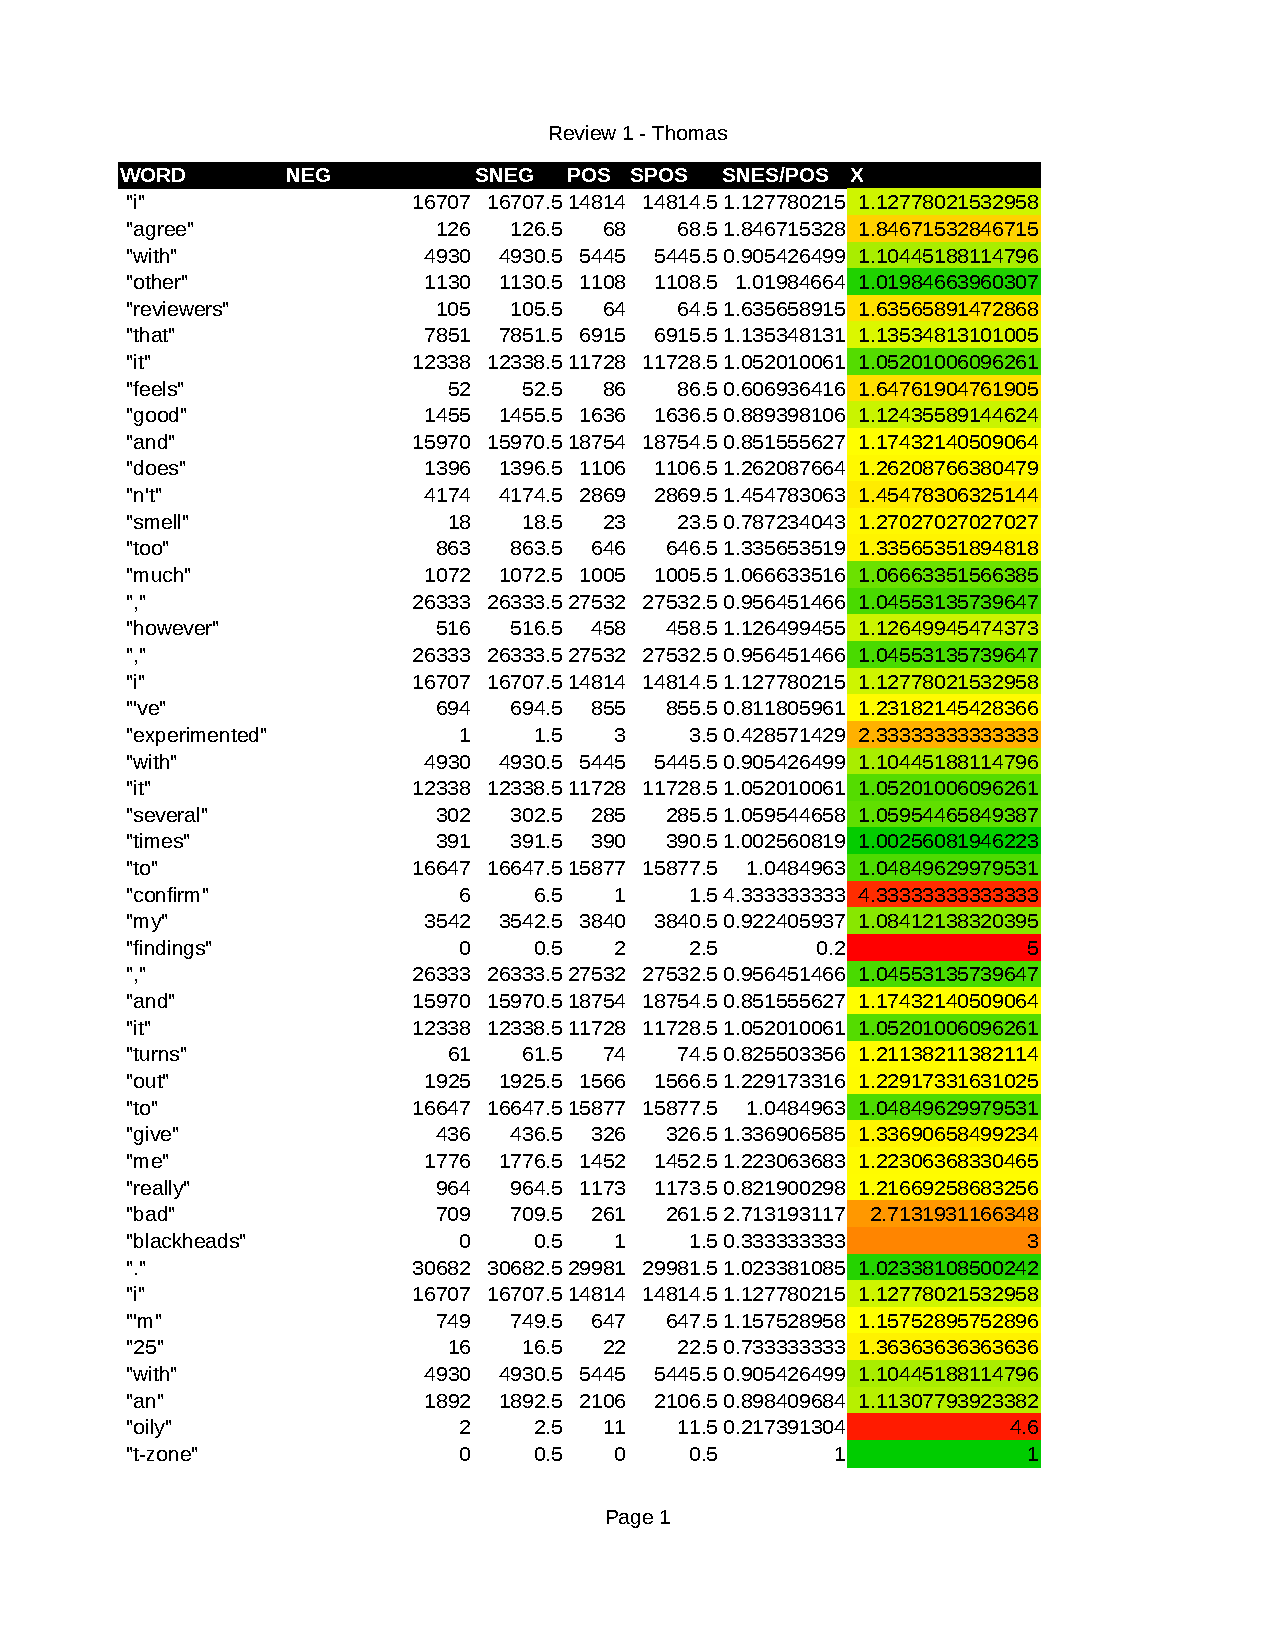
\includepdf[pages=-]{review-1-data.pdf}
    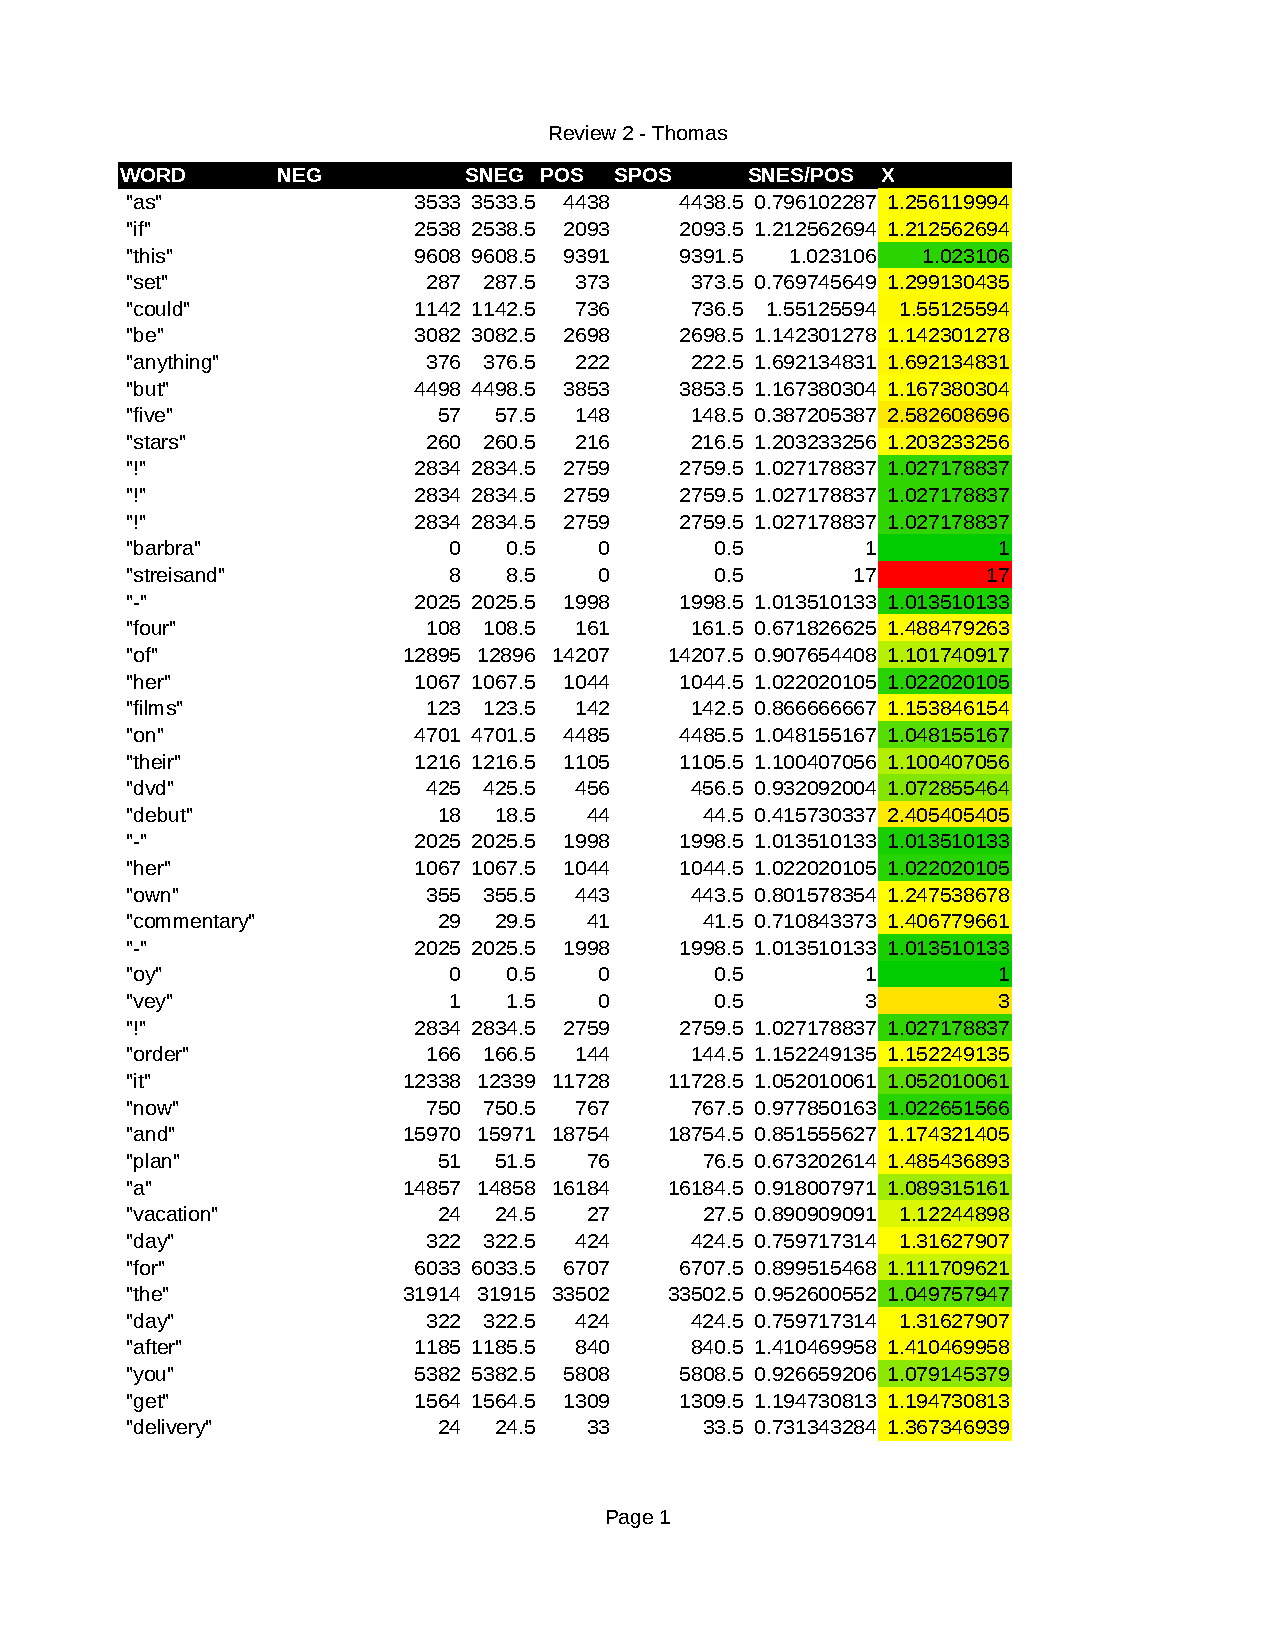
\includepdf[pages=-]{review-2-data.pdf}
    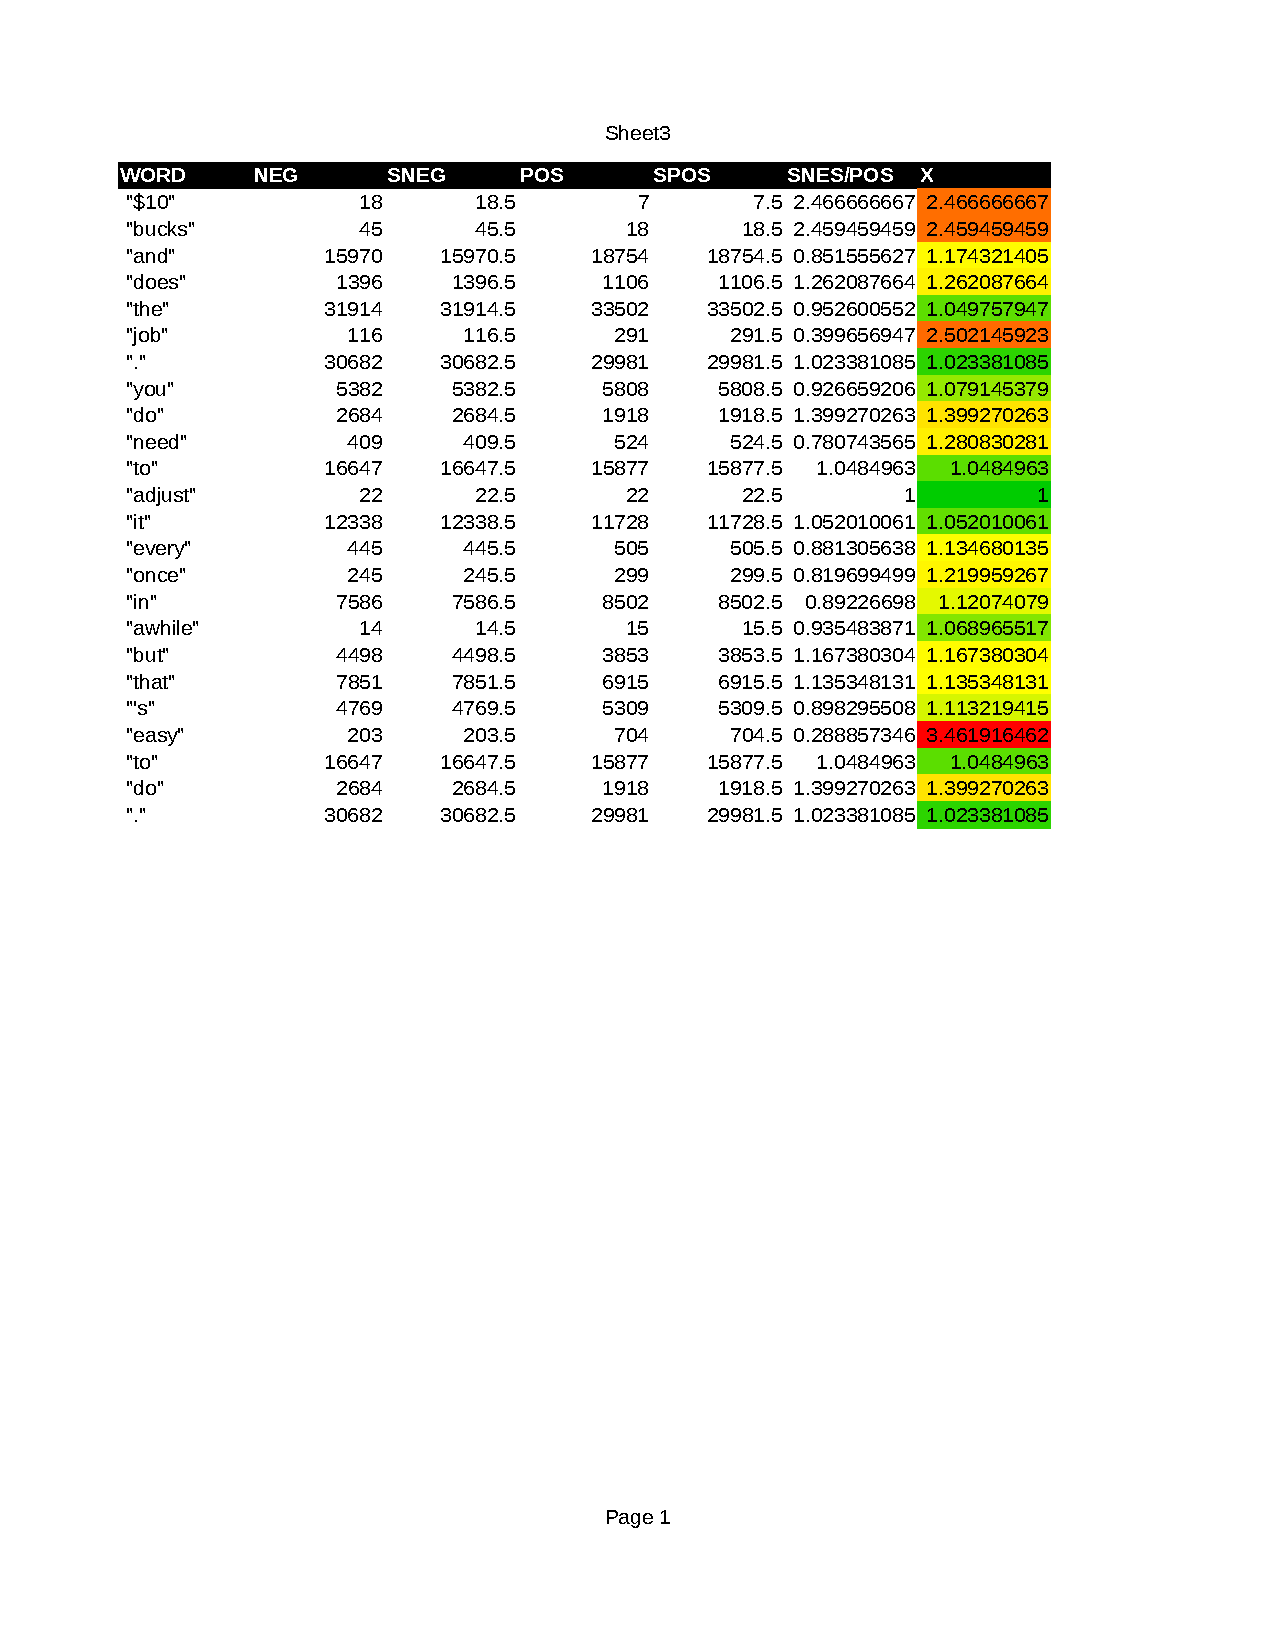
\includepdf[pages=-]{review-3-data.pdf}
\end{document}